% Document class
\documentclass[
  11pt,
  a4paper,
  oneside
]{book}

% Fonts
\usepackage[]{times}
\usepackage{setspace}
\setstretch{1.5}
\usepackage{amssymb,amsmath}
\usepackage[T1]{fontenc}
\usepackage[utf8]{inputenc}
\usepackage{textcomp} % provides euro and other symbols
\usepackage{lipsum}
\usepackage{import}

% remove Chapter N from Chapters
\usepackage{titlesec}
\titleformat{\chapter}[display]
  {\normalfont\bfseries}{}{0pt}{\Huge}
\titlespacing*{\chapter}{0pt}{0pt}{40pt} % minimize space between heading and top of the page

\titleformat{\chapter}[hang]{\Huge\bfseries}{\thechapter{. }}{0pt}{\Huge\bfseries} %creates number in front of chapter

% Use upquote if available, for straight quotes in verbatim environments
\IfFileExists{upquote.sty}{\usepackage{upquote}}{}

% Use microtype if available, for a nicer text
\IfFileExists{microtype.sty}{
  \usepackage[]{microtype}
  \UseMicrotypeSet[protrusion]{basicmath} % disable protrusion for tt fonts
}{}

% Language. Change to ngerman if you write in German
\usepackage[ngerman]{babel}

% Margins
\usepackage[margin=1in]{geometry}

% Paragraphs
\makeatletter
\setlength{\parindent}{0pt}
\setlength{\parskip}{6pt plus 2pt minus 1pt}
\makeatother
\usepackage{xcolor}

% Links
\usepackage[hyphens]{url}
\IfFileExists{xurl.sty}{\usepackage{xurl}}{} % add URL line breaks if available
\usepackage[unicode=true]{hyperref}
\hypersetup{
  pdftitle={Thesis template}, % CHANGE ME
  pdfauthor={Insert Your Name},
  pdfborder={0 0 0}, % CHANGE ME
  colorlinks=true,
  linkcolor=.,
  citecolor=.,
  urlcolor=blue,
  breaklinks=true}
\urlstyle{same}  % don't use monospace font for urls

% Graphics
\usepackage{graphicx}
\graphicspath{ {./img/} }

% Redefines (sub)paragraphs to behave more like sections
\ifx\paragraph\undefined\else
  \let\oldparagraph\paragraph
  \renewcommand{\paragraph}[1]{\oldparagraph{#1}\mbox{}}
\fi
\ifx\subparagraph\undefined\else
  \let\oldsubparagraph\subparagraph
  \renewcommand{\subparagraph}[1]{\oldsubparagraph{#1}\mbox{}}
\fi

% plain: Page numbers in the footer. Use "fancy" for nice headers.
\usepackage{fancyhdr}
\pagestyle{plain}

% Bibliography
\usepackage{natbib}

% Start of the document
\begin{document}
\frontmatter

% Title page % CHANGE ME
\begin{titlepage}
\begin{center}
 
\includegraphics[width=0.5\textwidth]{tuc}\\ % Logo
 {\huge\bfseries Your title\\[5pt] } % Title and optional subtitle
 \vspace{1.5cm}
 {\Large\bfseries Hugo Wienhold}\\[5pt] % Author
 \vspace{2cm}
% {Submitted in partial fulfilment for the award of the degree of} \\[2cm]
{zum Erlangung des akademischen Grades} \\[2cm]
\textsc{\Large{{B.Sc. Informatik}}} \\[5pt] % Degree
 \vfill
% {Department of Computer Science}\\[5pt] % Departement
{Fakultät für Informatik}\\[5pt] % Departement
% {Professorship for Artificial Intelligence}\\[5pt] % Professorship
{Professur Medieninformatik}\\[5pt] % Professorship
 \vfill
\emph{Supervisors:}\\ % Supervisors
% \emph{Gutachter:}\\ % Supervisors
Dr. Thomas Wilhelm-Stein \\
 % Dr.~habil. Julien Vitay \\
 \vfill
{\today} % Date of submission
\end{center}
\end{titlepage}

\chapter*{Abstract}
\label{sec:abstract}
Citations use \texttt{cite} inside a sentence (\cite{Vitay2014} showed that...) or \texttt{citep} as a reference \citep{Villagrasa2018}.\\


% Table of Contents
{
\setcounter{tocdepth}{3}
\hypersetup{linkcolor=black}
\tableofcontents
}

% Optional: list of figures and tables
% \listoffigures
% \listoftables

% Content
\mainmatter

\chapter*{Einleitung}
\addcontentsline{toc}{chapter}{Einleitung}
\label{sec:introduction}

% includes für die Einführung


\chapter{Grundlagen der Ladegeschwindigkeiten von Webseiten}
\label{sec:grundlagen_der_ladegeschwindigkeiten_von_websiten}

\section{Definitionen und Ansätze}
\label{sec:definitionen_und_ansatze}
Die Ladegeschwindigkeit einer Website, auch als Seitenladezeit oder Seitengeschwindigkeit bezeichnet, ist ein zentraler Aspekt der Performance einer Webseite und spielt eine entscheidende Rolle für die Nutzererfahrung sowie die Suchmaschinenoptimierung (SEO) (Wilkinson, 2024). Verschiedene Definitionen betonen dabei unterschiedliche Nuancen des Begriffs.

\subsection{Definition der Ladegeschwindigkeit}
\label{sec:definition_der_ladegeschwindigkeit}
Elbeyoglu (2021) beschreibt die Seitenladezeit als die Zeitspanne, die erforderlich ist, damit alle Informationen auf einer Webseite vollständig angezeigt werden. Diese Ladezeit wird auch als Seitengeschwindigkeit bezeichnet und misst die Effizienz des Ladevorgangs. Der Fokus liegt hier auf der Vollständigkeit der Darstellung der Seite, was eine benutzerorientierte Perspektive betont.

Die Definition von Page Load Time (2023) beschreibt die Seitenladezeit als die Dauer, die eine Webseite benötigt, um vollständig zu laden, gemessen in Sekunden. Zwar wird hier die vollständige Ladung als zentraler Punkt genannt, jedoch wird auch die quantitative Messbarkeit der Ladezeit betont, wodurch die Ladezeit als wichtiger Indikator für die Leistungsfähigkeit einer Webseite hervorgehoben wird.

Wilkinson (2024) legt den Schwerpunkt auf die Schnelligkeit des Ladevorgangs. Nach dieser Definition misst die Seitengeschwindigkeit, wie schnell der Inhalt einer Seite geladen wird, wobei der Begriff Ladegeschwindigkeit synonym verwendet wird. Dieser Ansatz konzentriert sich stärker auf die Effizienz des Ladevorgangs, ohne die vollständige Anzeige des gesamten Inhalts als zwingenden Maßstab zu betrachten.

Die Quelle „What Is Website Loading Speed?“ (o. D.) bietet eine weitere Betrachtung, indem sie die Ladegeschwindigkeit als die Zeit beschreibt, die benötigt wird, um den gesamten Inhalt einer Website auf dem Gerät des Nutzers darzustellen, nachdem diese durch Eingabe einer URL, das Anklicken eines Links oder eine Weiterleitung aufgerufen wurde. Diese Definition integriert explizit die Nutzerperspektive, indem der gesamte Prozess von der Benutzeraktion bis zur vollständigen Anzeige der Inhalte auf dem Endgerät des Nutzers beschrieben wird.

\subsection{Der Ladeprozess als mehrstufige Einheit}
\label{sec:der_ladeprozess_als_mehrstufige_einheit}
Web.dev, eine von Google gestützte Seite, bietet einen weiteren Ansatz zur Ladegeschwindigkeit. Anstey und Pavic (2019) betrachten das Laden einer Webseite nicht als einen einzelnen Moment, sondern als einen mehrstufigen Prozess. Dieser Ansatz hebt hervor, dass einzelne Metriken, wie etwa die DOMContentLoaded-Zeit, kein vollständiges Bild des Nutzererlebnisses vermitteln können. Stattdessen wird die Ladegeschwindigkeit in drei Etappen mit vier Messwerten unterteilt.

Die erste Etappe lautet "Is it happening?" und überprüft, ob die Navigation erfolgreich begonnen hat und ob der Server reagiert. In dieser Etappe werden die Metriken "First Paint" und "First Contentful Paint" gemessen, die die Zeit beschreiben, bis etwas Sichtbares, sei es ein Bild oder Text, auf der Seite erscheint.

Die zweite Etappe heißt "Is it useful?" und markiert den Zeitpunkt, an dem genügend Inhalt geladen ist, sodass sich der Nutzer sinnvoll mit der Seite beschäftigen kann. Dies ist der Moment, in dem erkennbar wird, ob die Website für den Nutzer von Interesse ist. Diese Phase wird durch die Metrik "First Meaningful Paint" beschrieben.

Die dritte Etappe heißt "Is it usable?" und beschreibt den Zeitpunkt, ab dem der Nutzer tatsächlich mit der Webseite interagieren kann. Hierbei kommt die Metrik "Time to Interactive" zum Einsatz, die misst, wann die Webseite  funktionsfähig ist und  interaktiven Elemente genutzt werden können.

Nach diesen drei Etappen kann der initiale Ladeprozess als abgeschlossen betrachtet werden. Optional kann jedoch eine vierte Etappe hinzugefügt werden: "Is it delightful?". Diese beschreibt die Qualität der Nutzung der Webseite, wobei Faktoren wie reibungslose Nutzung, das Fehlen von Verzögerungen und eine flüssige Bedienung im Vordergrund stehen. Auch hier werden weitere spezifische Messwerte benötigt, um die Benutzerfreundlichkeit und die natürliche Interaktion zu bewerten.

Insgesamt wird aus diesen verschiedenen Definitionen deutlich, dass die Ladegeschwindigkeit sowohl technische Aspekte der Performance als auch die Benutzererfahrung umfasst. Sie beeinflusst direkt die Zufriedenheit der Nutzer und kann sich direkt auf das Engagement und die Wiederkehrwahrscheinlichkeit auswirken.




\section{Einflussfaktoren auf die Ladegeschwindigkeit und deren Lösungen}
\label{sec:einflussfaktoren_auf_die_ladegeschwindigkeit_und_deren_lösungen}




\section{Tests für Ladegeschwindigkeiten}
\label{sec:test_fur_ladegeschwindigkeiten}
% 3-4 Unterschiedliche Testingtools für die Ladegeschwindigkeit aufführen

% auf die unterschiedlichen Arten von Tests 


\subsection{GT Metrix}
\label{sec:gt_metrix}
GT Metrix (GTMetrix | Website Performance Testing and Monitoring, o. D.) ist ein automatisiertes Tool, das speziell für die Analyse der Ladegeschwindigkeit und der allgemeinen Performance von Websites entwickelt wurde. GT Metrix bietet eine detaillierte Analyse, die es ermöglicht, Schwachstellen zu identifizieren und gezielte Verbesserungen vorzunehmen.

Das Tool ist in einer kostenlosen und einer kostenpflichtigen Version verfügbar, wobei bereits die kostenlose Version zahlreiche Funktionen bietet. Ein besonders wichtiger Bestandteil der Analyse sind die so genannten "Core Web Vitals", die im Suchalgorithmus von Google eine entscheidende Rolle spielen. Diese Metriken, die die Ladezeit, die Interaktivität und die visuelle Stabilität einer Seite bewerten, sind entscheidend für die Platzierung einer Website in den Suchergebnissen von Google. GT Metrix erstellt nach jedem Test einen umfassenden Bericht, der sowohl die Performance der Website als auch ihre strukturellen Merkmale aufzeigt. Der Performance Score ist ein Maß für die Performance der Website aus Sicht des Nutzers, der Structure Score ein Maß dafür, wie gut die Website für eine optimale Performance strukturiert ist.

Zusätzlich bietet GT Metrix eine visuelle Darstellung der Ladegeschwindigkeit in Form der "Speed Visualisation". Dabei wird der Ladevorgang der Seite in Intervallen dargestellt und wichtige Leistungsindikatoren während des Ladevorgangs hervorgehoben. So kann der Nutzer den Ladevorgang besser nachvollziehen und erkennen, welche Bereiche der Seite besonders viel Zeit in Anspruch nehmen. Darüber hinaus listet das Tool im Abschnitt "Top Issues" strukturelle Probleme auf, die zu den größten Leistungsverlusten führen, so dass die größten Schwachstellen der Website leicht identifiziert werden können. Die "Page Details" sind eine Aufschlüsselung der Anfragen, die während des Seitenaufrufs gestellt wurden, einschließlich der Anzahl und Größe dieser Anfragen. Diese detaillierte Übersicht gibt Aufschluss darüber, welche Elemente der Website den Seitenaufbau verlangsamen können.

Basierend auf der durchgeführten Analyse liefert das Tool auch konkrete Optimierungsvorschläge. Diese Vorschläge sind in einem eigenen GT Metrix-Bereich zusammengefasst und helfen dem Nutzer, gezielt an den identifizierten Schwachstellen zu arbeiten. Die verschiedenen Reiter für Performance, Struktur und weitere Bereiche ermöglichen eine detaillierte Betrachtung der Testergebnisse. Besonders praktisch ist die Möglichkeit, die Website-Performance aus verschiedenen geografischen Regionen zu testen. Sieben globale Standorte ermöglichen es dem Nutzer zu sehen, wie schnell seine Seite in verschiedenen Teilen der Welt geladen wird.

Ein weiteres nützliches Feature der kostenlosen Version ist die Möglichkeit, automatisierte Tests zu planen, die täglich, wöchentlich oder monatlich ausgeführt werden. Damit lassen sich langfristige Trends wie die Entwicklung der Web Vitals, des GT Metrix Grades, der Performance- und Struktur-Scores, der Seiten- und Dateigrößen sowie der Anzahl der Requests verfolgen. Auf diese Weise ist der Website-Betreiber in der Lage, die Performance seiner Website über einen längeren Zeitraum zu beobachten und frühzeitig auf Veränderungen zu reagieren.

Ein weiterer wichtiger Bestandteil der Analyse ist das Wasserfalldiagramm, das den Ladeprozess der Seite detailliert darstellt und lange oder fehlerhafte Requests hervorhebt. Diese visuelle Darstellung hilft, Engpässe im Ladeprozess zu identifizieren und gezielt Verbesserungen vorzunehmen. Darüber hinaus bietet GT Metrix die Möglichkeit, Tests mit und ohne Adblocker durchzuführen, um zu sehen, wie Werbung die Ladezeiten beeinflusst. Eine Verbindungsdrosselungsfunktion ermöglicht es, die Performance der Website bei unterschiedlichen Internetgeschwindigkeiten zu simulieren. Weitere Funktionen der kostenlosen Version sind Benachrichtigungen, wenn die Performance unter ein bestimmtes Niveau fällt, und die Möglichkeit, den Ladevorgang der Website aus Sicht des Nutzers per Video Playback zu sehen.

Die kostenpflichtige Version von GT Metrix erweitert den Funktionsumfang der kostenlosen Version erheblich und bietet zahlreiche zusätzliche Tools, die insbesondere für fortgeschrittene Nutzer und Unternehmen nützlich sind. Eine der wichtigsten Erweiterungen ist das Mobile Testing, mit dem die Performance einer Website auf über 40 verschiedenen Mobilgeräten getestet werden kann, darunter beliebte Modelle wie iPhone, Samsung Galaxy und Google Pixels. Dies ist wichtig, da immer mehr Nutzerinnen und Nutzer von mobilen Geräten aus auf Websites zugreifen und eine optimale Performance auf diesen Geräten unerlässlich ist.

Darüber hinaus bietet die kostenpflichtige Version 15 zusätzliche globale Standorte, die es ermöglichen, die Ladegeschwindigkeit und Performance der Website in noch mehr geografischen Regionen zu testen. Dies erweitert die Reichweite im Vergleich zu den sieben Standorten der kostenlosen Version erheblich und ist besonders für international ausgerichtete Websites hilfreich, die ihre Nutzer in verschiedenen Teilen der Welt erreichen möchten.

Ein weiteres leistungsstarkes Feature ist die stündliche Überwachung der Website-Performance. Damit lassen sich detaillierte Informationen darüber gewinnen, zu welchen Tageszeiten die größten Leistungseinbußen auftreten. Dies ermöglicht eine genauere Diagnose von Problemen und gibt Einblick in das Nutzerverhalten zu unterschiedlichen Zeiten.

Darüber hinaus bietet die kostenpflichtige Version eine unbegrenzte Anzahl von Tags, die zur Kategorisierung und Sortierung von Fehlern und Berichten verwendet werden können. Diese Funktion ist besonders nützlich, um wiederkehrende Probleme zu verwalten und zu organisieren oder um einen systematischen Überblick über Bereiche mit Verbesserungspotenzial zu erhalten. Weitere erweiterte Analyseoptionen umfassen die Anpassung der Bildschirmauflösung und der Internetgeschwindigkeit, um noch genauere Tests durchzuführen und die Ladezeiten unter verschiedenen Bedingungen zu simulieren.

Ein zusätzlicher Vorteil der Premium-Version ist die längere Speicherung der Berichte, die einen tieferen Einblick in die vergangene Leistung der Website bietet und langfristige Trends besser sichtbar macht. Für Entwickler, die in einer Entwicklungs- oder Staging-Umgebung arbeiten, bietet die kostenpflichtige Version auch die Möglichkeit, einen eigenen DNS zu verwenden. Damit können Hostnamen und IP-Adressen für spezifische Testzwecke angepasst werden.

Ein weiterer Vorzug der kostenpflichtigen Version ist der priorisierte Zugriff auf die Warteschlange der Benutzeranfragen, was eine schnellere Bearbeitung der Tests und eine schnellere Bereitstellung der Ergebnisse ermöglicht. Die Möglichkeit des weltweiten Monitorings und der Download kompletter PDF-Berichte bieten eine umfassende Dokumentation der Testergebnisse, die leicht weitergegeben und archiviert werden kann.

Ein weiteres zentrales Feature der Premium-Version ist die API-Funktionalität. Diese ermöglicht es Entwicklern und Unternehmen, GT Metrix direkt in ihre eigenen Systeme zu integrieren und automatisierte Tests sowie detaillierte Analysen durchzuführen. Mit der API können Performancetests ohne manuelle Eingriffe durchgeführt werden, was insbesondere bei größeren Projekten oder für ein regelmäßiges Monitoring von Vorteil ist. Mit Hilfe der API kann der gesamte Prozess automatisiert und an die individuellen Anforderungen angepasst werden. Dies spart Zeit und Ressourcen und stellt sicher, dass die Performance der Website kontinuierlich überwacht und optimiert wird. 



\subsection{Tool 2}
\label{sec:}


\subsection{Google PageSpeed Insights}
\label{sec: pagespeed_insights}

Google PageSpeed Insights basiert auf zwei verschiedenen Arten von Daten, den Felddaten und den Labordaten, die jeweils unterschiedliche Aspekte der Website-Leistung aufzeigen und zusammen ein vollständiges Bild des Nutzererlebnisses und der Ladegeschwindigkeit ergeben.

Die Felddaten in Google PageSpeed Insights stammen aus dem Chrome User Experience Report (CrUX) und sind sehr nützlich, da sie auf echten Nutzerdaten basieren, die weltweit in Chrome-Browsern erfasst wurden. Diese Daten spiegeln die tatsächliche Nutzererfahrung wieder, da sie aus realen Interaktionen von Nutzern stammen, die die Website besucht haben. Dies bedeutet, dass die Daten im Gegensatz zu simulierten Labortests ein authentisches Bild davon vermitteln, wie sich eine Website in verschiedenen Netzwerken, auf verschiedenen Geräten und unter verschiedenen Bedingungen verhält. Die Datenerhebung erfolgt in regelmäßigen Abständen, konkret alle 28 Tage, so dass die Ergebnisse kontinuierlich aktualisiert werden.

Voraussetzung für die Datenerhebung mit CrUX ist allerdings, dass die analysierte Website öffentlich zugänglich ist und über eine ausreichend große Nutzerbasis verfügt. Nur so kann eine repräsentative Stichprobe erreicht werden. Eine genaue Mindestzahl an Besuchern wird von Google nicht genannt, es wird jedoch sichergestellt, dass genügend Daten für eine valide Analyse zur Verfügung stehen. Ein weiterer wichtiger Aspekt der Felddaten ist, dass sie zwischen mobilen Geräten und Computern unterscheiden, um die Performance in beiden Nutzungsszenarien genau abbilden zu können.

\begin{figure}
    \centering
    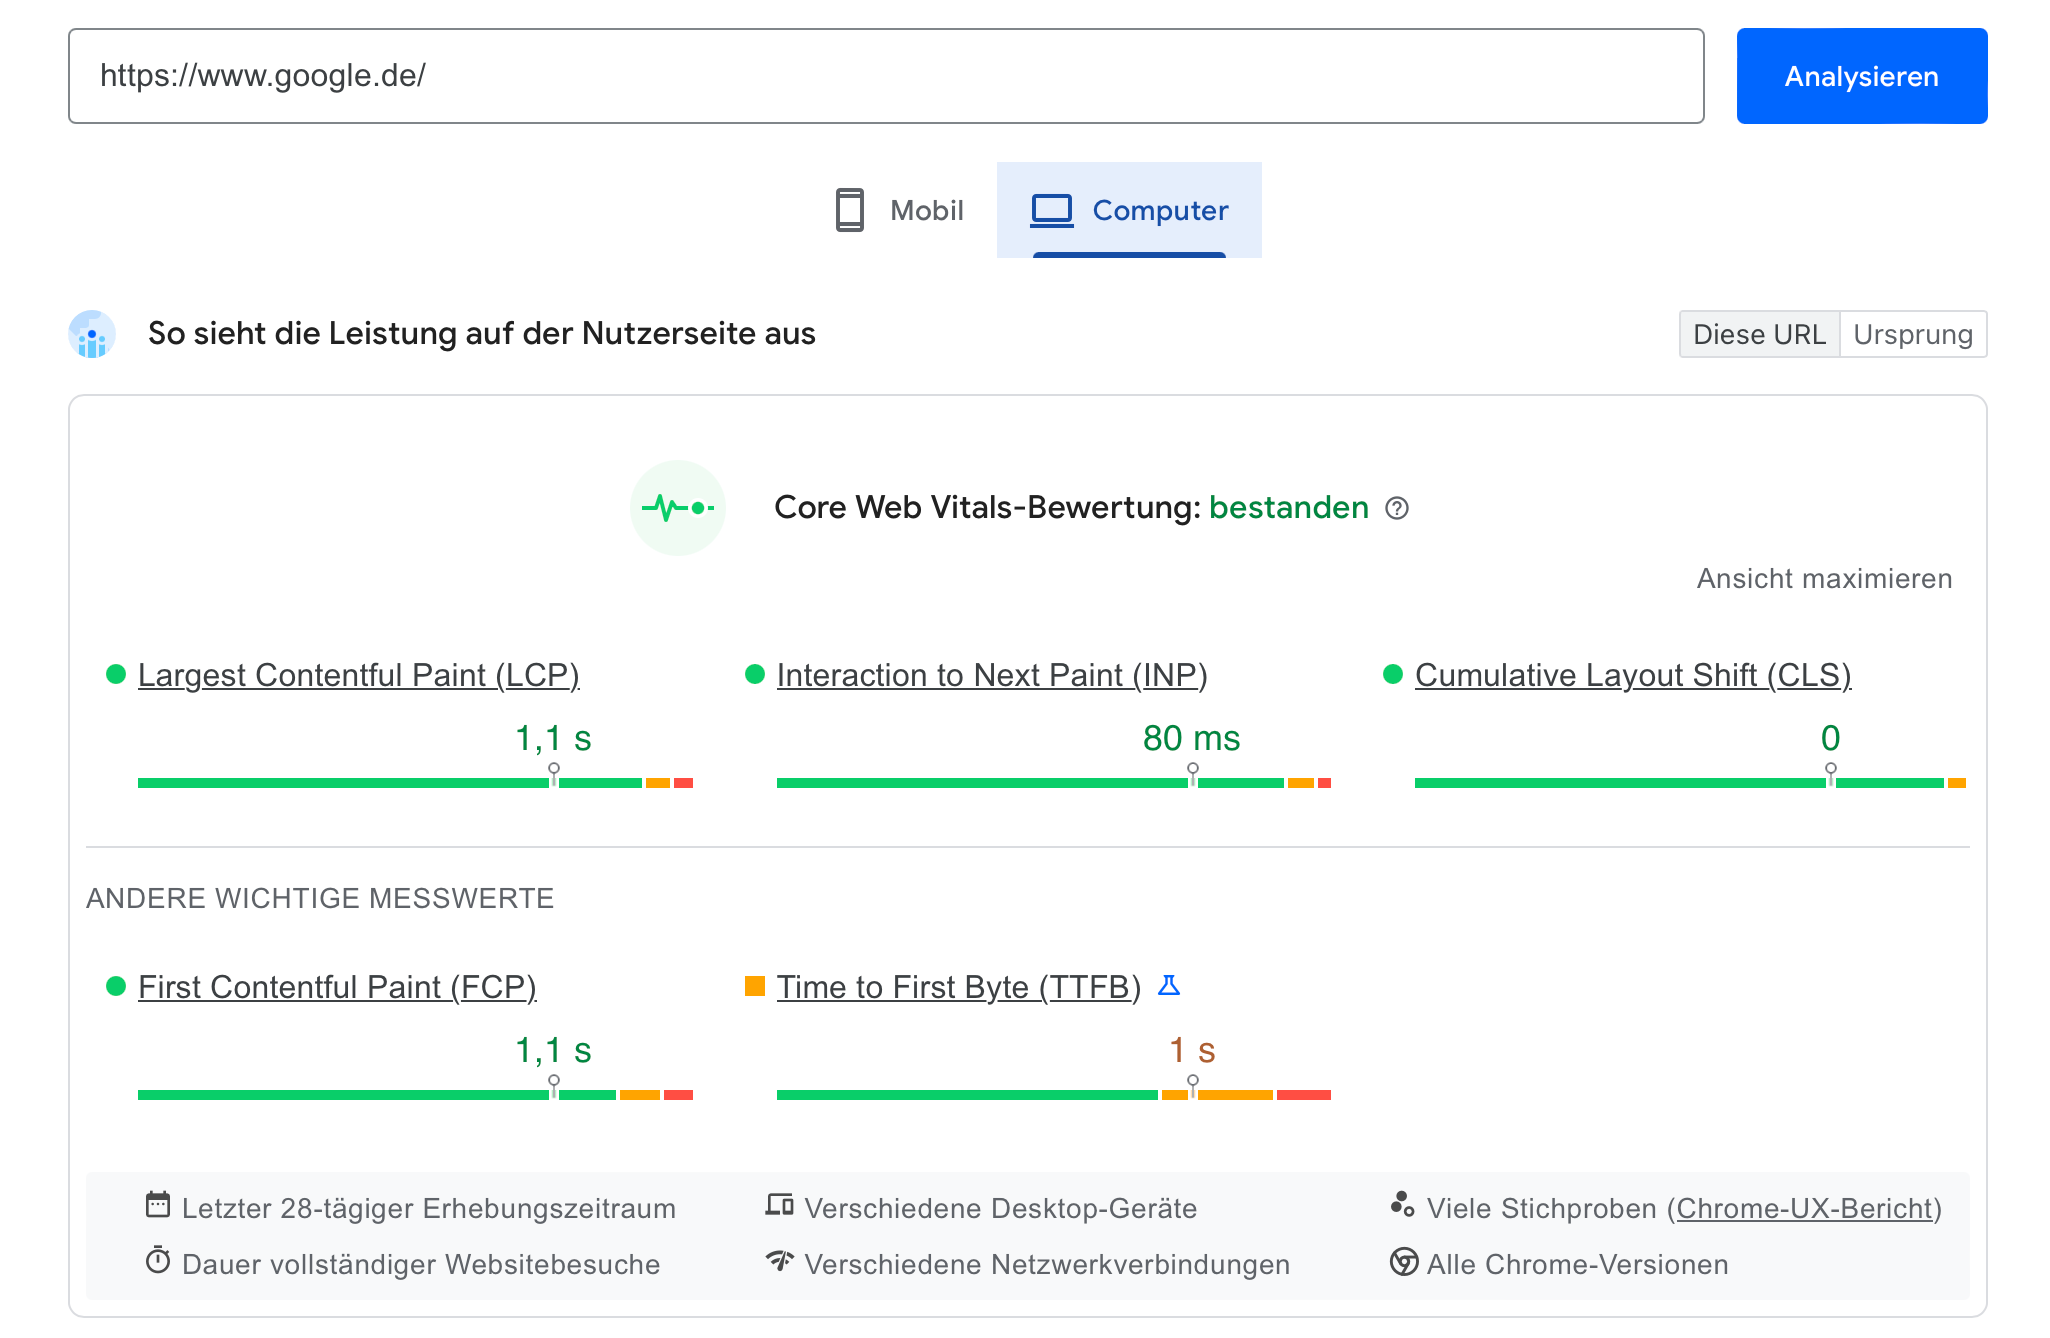
\includegraphics[width=1 \textwidth]{psi_user}
    \caption{PageSpeed Insights Übersicht der CrUX-Daten am Beispiel von https://www.google.de/}
    \label{fig:crux_data}
\end{figure}

Für die Analyse der Website-Performance werden mehrere Leistungskennzahlen gemessen, die wichtige Informationen über die Ladegeschwindigkeit und das Nutzererlebnis liefern. Eine der zentralen Metriken ist "Largest Contentful Paint" (LCP), welche den Zeitpunkt misst, zu dem der größte sichtbare Inhalt einer Seite geladen wird. Dies ist besonders relevant, da die Nutzer erwarten, dass sie schnell zum Hauptinhalt einer Seite gelangen. Ein weiterer wichtiger Indikator ist Interaction to Next Paint (INP), welcher die Reaktionsfähigkeit der Seite auf Nutzerinteraktionen während der Nutzung misst. Diese Metrik gibt Aufschluss darüber, wie gut die Seite auf Benutzereingaben reagiert, was ein wichtiger Faktor für die Benutzererfahrung ist.

Cumulative Layout Shift (CLS) ist eine Metrik, die Layoutverschiebungen während des Seitenladens misst. Unerwartete Bewegungen von Inhalten, wie das Verschieben von Text oder Bildern, können das Nutzererlebnis negativ beeinflussen, daher ist der CLS-Wert wichtig, um die visuelle Stabilität der Seite zu beurteilen. Zusätzlich wird der First Contentful Paint (FCP) gemessen, der den Zeitpunkt angibt, zu dem der Nutzer den Inhalt der Seite zum ersten Mal sieht. Ein schneller FCP sorgt für einen positiven ersten Eindruck, da der Nutzer sofort eine visuelle Rückmeldung erhält, dass die Seite geladen wird. Die Time to First Byte (TTFB) gibt schließlich an, wie lange es dauert, bis der Browser die ersten Daten vom Server erhält. Eine niedrige TTFB ist ein Zeichen für einen schnellen Server und eine effiziente Backend-Infrastruktur.

Die Lab-Daten in Google PageSpeed Insights stammen aus Lighthouse, einem Open-Source-Tool von Google, das Webseiten unter kontrollierten Bedingungen analysiert. Im Gegensatz zu den Field-Daten, die reale Nutzerdaten wiederspiegeln, werden die Lab-Daten in einer simulierten Umgebung erhoben. Das bedeutet, dass die Performance der Seite unter bestimmten, vordefinierten Bedingungen getestet wird. Dies geschieht durch die Emulation von Geräten und Netzwerkbedingungen, um möglichst realitätsnahe Szenarien zu simulieren. So wird beispielsweise ein Moto G Power als Standardgerät für mobile Tests verwendet und die Netzwerkgeschwindigkeit künstlich gedrosselt, um zu simulieren, wie die Seite unter langsameren Verbindungen geladen wird.

Lab-Daten liefern eine Momentaufnahme der aktuellen Leistung einer Website und konzentrieren sich auf die Seite, wie sie zum Zeitpunkt der Messung existiert. Im Gegensatz zu den Felddaten wird hier nicht auf historische Nutzerdaten zurückgegriffen, sondern die jeweilige URL wird einmalig getestet. Es werden nur die explizit eingegebenen URLs analysiert, nicht aber die angrenzenden Seiten, wie es beispielsweise bei CrUX der Fall ist.

Die Ergebnisse der Lab-Daten werden in vier Kategorien eingeteilt: Performance, Accessibility, Best Practices und SEO (Search Engine Optimization). Für die Analyse der Ladegeschwindigkeit ist vor allem die Kategorie Performance relevant. In dieser Kategorie bewertet PageSpeed Insights die Performance der Seite anhand von fünf wichtigen Schlüsselmetriken, die in einen Performance-Score einfließen.

\begin{figure}
    \centering
    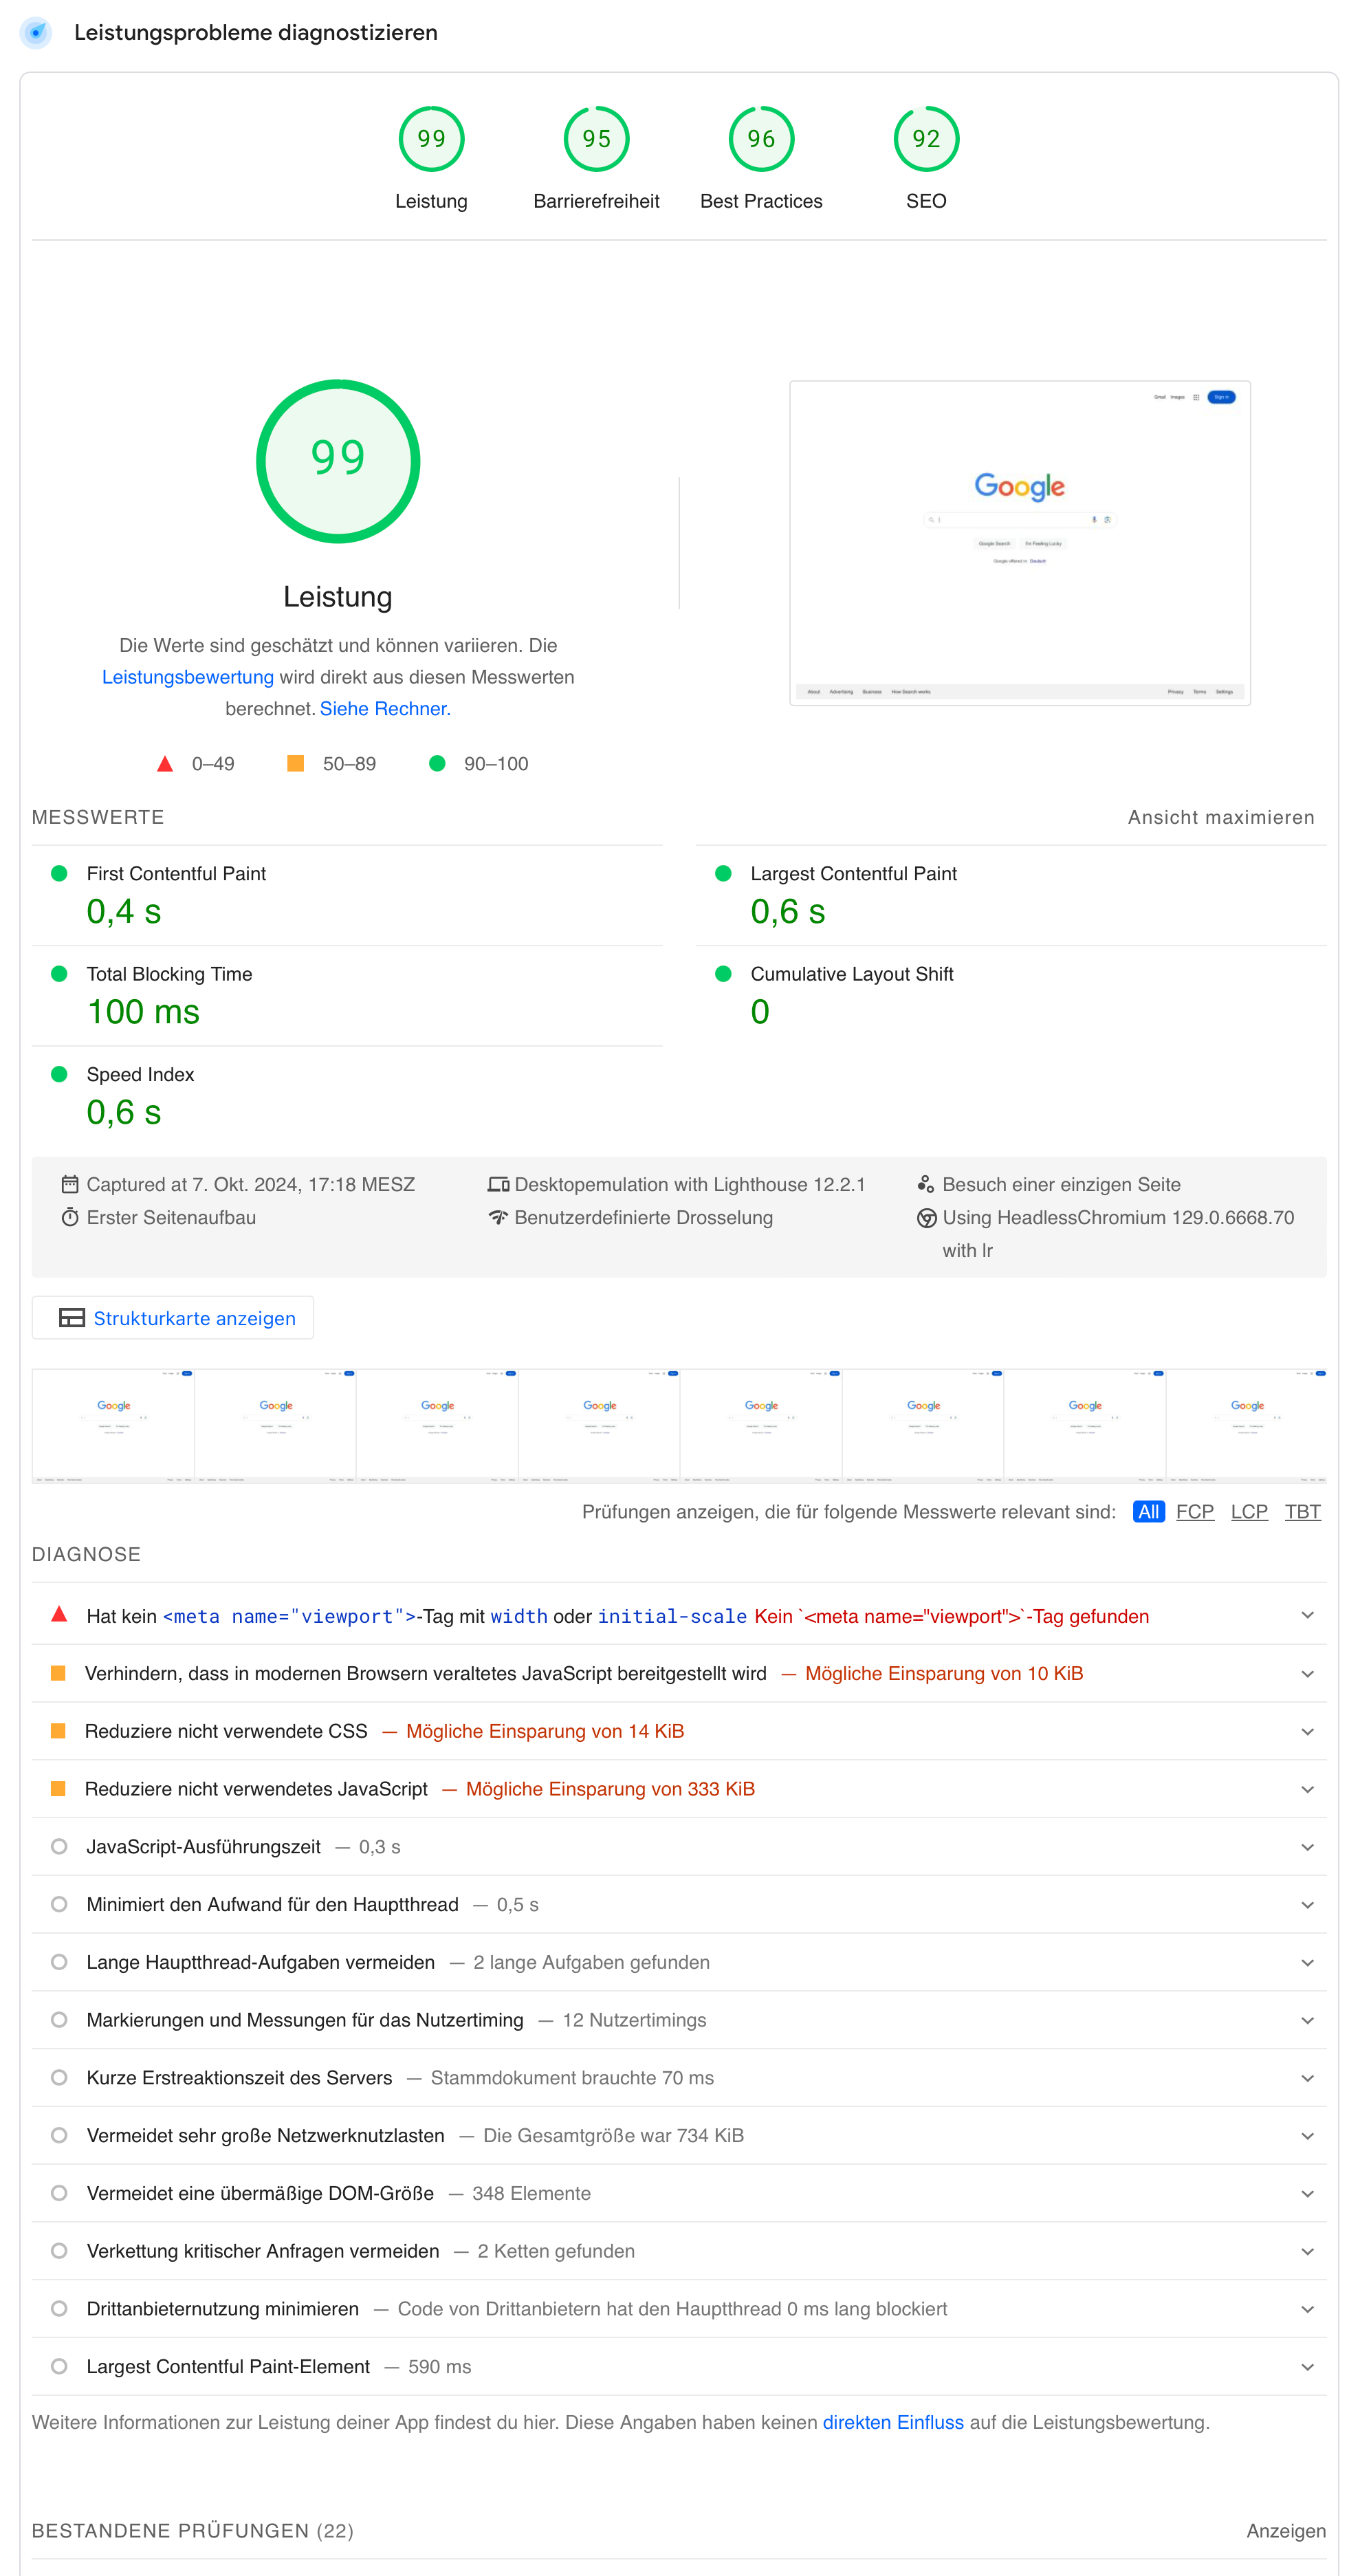
\includegraphics[height=0.9\textheight]{psi_performance}
    \caption{PageSpeed Insights Übersicht der Lab-Daten am Beispiel von https://www.google.de/}
    \label{fig:psi_performance}
\end{figure}

Zu diesen Metriken gehört wie bei CrUX  First Contentful Paint (FCP), Largest Contentful Paint (LCP) und Cumulative Layout Shift (CLS), welche nochmals zum Zeitpunkt der Anfrage ermittelt werden. 

Eine weitere wesentliche Metrik ist die Total Blocking Time (TBT). Sie misst die Summe der Zeiträume, in denen die Seite blockiert ist und nicht auf Benutzerinteraktionen reagiert. Dieser Wert ist besonders wichtig, um festzustellen, ob die Seite in der Lage ist, schnell auf Benutzereingaben zu reagieren, was einen großen Einfluss auf die allgemeine Benutzererfahrung hat. Schließlich gibt es noch den Speed Index, der angibt, wie schnell der Inhalt einer Seite insgesamt angezeigt wird.

Zusätzlich zu diesen Kernmetriken bietet Lighthouse auch detaillierte Informationen über die Seitenstruktur und visualisiert den Aufbau der Website in einer Reihe von Bildern, die zeigen, wie die Seite Schritt für Schritt geladen wird. Diese visuelle Darstellung kann helfen, Engpässe im Ladeprozess zu identifizieren. Zusätzlich gibt es den Reiter Diagnose, der mögliche Probleme auflistet und Einsparpotenziale aufzeigt. Diese Diagnosehinweise enthalten  konkrete Vorschläge zur Verbesserung der Ladegeschwindigkeit und zur Behebung von Schwachstellen.

Abgerundet wird die Analyse durch bestandene Tests, die zeigen, welche Tests die Seite ohne Probleme bestanden hat. 

Ein weiterer großer Vorteil von Google PageSpeed Insights ist die Verfügbarkeit einer kostenlosen API, über die Entwickler und Website-Betreiber automatisiert auf die Messwerte zugreifen können. Diese API ermöglicht es, regelmäßige Performance-Tests durchzuführen, ohne manuell auf die PageSpeed Insights-Website zugreifen zu müssen. Besonders nützlich ist die Möglichkeit, zusätzliche Daten wie Time to Interactive, DOM Size und Total Byte Weight abzufragen, um eine noch detailliertere Analyse der Performance durchzuführen. Mit einem API-Schlüssel können bis zu 240 Abfragen pro Minute bzw. 25.000 Abfragen pro Tag kostenlos durchgeführt werden.

PageSpeed Insights ist generell kostenlos und ohne Login für jeden zugänglich. Durch die Kombination von realen Nutzerdaten und Lab-Daten bietet Google PageSpeed Insights einen umfassenden und zuverlässigen Einblick in die Ladegeschwindigkeit und allgemeine Performance einer Website. In meiner empirischen Analyse im späteren Verlauf der Arbeit wird Google PageSpeed Insights als zentrales Tool verwendet, um die Ladegeschwindigkeit und Performance verschiedener Websites zu analysieren.



\chapter{Website Usability}
\label{sec:website_usability}

% was ist Usability eigentlich und warum ist das wichtig

\section{Definition Usability}

\section{Bedeutung der Ladegeschwindigkeit für die Usability}
\label{sec:bedeutung_der_ladegeschwindigkeit_fur_die_usability}

\section{HTML-Tags und die Auswirkung auf die Usability}
\label{htmltags_und_die_auswirkung_auf_die_usability}

\section{Usability-Tests}
\label{sec:usabilitytests}

% Tool / Websiten / Unternehmen die Usability Test anbieten

% auf die unterschiedlichen Arten von Tests eingehen -> automatisiert / Expertentests / Usertest
\subsection{Automatisierte Tools zur Bewertung der Usability von Websites - SEOptimiser}
\label{sec:automatisierte_tools_zur_bewertung_der_usability_von_websites_seooptimiser}

SEOptimiser ist ein automatisiertes Tool, das zur Bewertung der Usability von Websites eingesetzt wird und in der Studie "A Review of Automated Website Usability Evaluation Tools: Research Issues and Challenges" von Namaoun et al. (2021) analysiert wurde. Das Tool wurde entwickelt, um Webdesigner und Website-Betreiber bei der Untersuchung der Usability, User Experience (UX) und Suchmaschinenoptimierung (SEO) ihrer Websites zu unterstützen. SEOptimiser geht über einfache Diagnosen hinaus und liefert spezifische, umsetzbare Empfehlungen zur Verbesserung der Website-Qualität.

Das primäre Ziel von SEOptimiser ist die Identifizierung von Usability- und Performance-Problemen sowie die Bereitstellung spezifischer Empfehlungen zur Verbesserung. Das Tool deckt dabei verschiedene Schlüsselbereiche ab, darunter SEO, Benutzerfreundlichkeit, Leistung, soziale Interaktion und Sicherheit. Diese umfassende Analyse macht SEOptimiser zu einer vielseitigen Lösung für die Webanalyse. Es ist bemerkenswert, dass SEOptimiser sechs verschiedene Dimensionen der Benutzerfreundlichkeit abdeckt, mehr als viele vergleichbare Tools. Zu den analysierten Bereichen gehören der Seiteninhalt, Ladegeschwindigkeit, Effizienz, Barrierefreiheit, Interaktivität und Navigation. Diese Dimensionen sind zentral für die User Experience, da sie die Art und Weise beeinflussen, wie Nutzer mit der Website interagieren. Zusätzlich bietet SEOptimiser detaillierte Einblicke in die SEO-Leistung, einschließlich der Seitenoptimierung, der Nutzung von Schlüsselwörtern und Meta-Beschreibungen.

SEOptimiser legt einen besonderen Fokus auf die Verbesserung der Usability und der User Experience. Die detaillierten Analysen helfen, Schwachstellen in der Benutzerführung und im Interface-Design zu identifizieren und konkrete Verbesserungsvorschläge zu machen. Zu den analysierten Dimensionen gehören Aspekte wie Navigation, Effizienz der Benutzerführung und Interaktivität der Website. Diese Faktoren sind entscheidend für eine gute UX, da sie sicherstellen, dass Nutzer die benötigten Informationen schnell finden, sich problemlos orientieren und insgesamt eine positive Interaktion mit der Website haben.

Die Empfehlungen von SEOptimiser zur Verbesserung der Usability konzentrieren sich auf konkrete Maßnahmen zur Optimierung der Benutzerinteraktion, zur Beseitigung technischer Probleme und zur Erhöhung der Zugänglichkeit. Im Gegensatz zu einigen anderen Tools, die nur allgemeine Bewertungen und vage Analysen bieten, liefert SEOptimiser detaillierte Diagnosen, die für Benutzer mit moderaten technischen Kenntnissen gut verständlich sind. Die Berichte des Tools sind übersichtlich gestaltet, was es auch für Nutzer ohne speziellen Hintergrund in der Website-Entwicklung einfacher macht, die Ergebnisse zu verstehen und anzuwenden.

Darüber hinaus unterstützt SEOptimiser die Verbesserung der User Experience, indem es mögliche Engpässe identifiziert, wie z. B. übergroße Seitenelemente, ineffiziente Programmierpraktiken oder mangelnde Barrierefreiheit, und konkrete Lösungen vorschlägt. Diese Art der Analyse ermöglicht es Website-Betreibern, die User Experience gezielt zu verbessern und sicherzustellen, dass alle Nutzer, unabhängig von ihren technischen Fähigkeiten oder Einschränkungen, eine möglichst positive Erfahrung machen.

Trotz seiner Stärken weist SEOptimiser auch Einschränkungen auf, insbesondere im Hinblick auf die theoretische Fundierung der Usability-Analysen. Ein Problem, das in der Studie festgestellt wurde, ist, dass SEOptimiser, ähnlich wie viele andere Tools, die theoretischen Grundlagen der Usability nicht vollständig in sein Analyse-Framework integriert. Das Tool bewertet eine begrenzte Anzahl von Usability-Dimensionen im Vergleich zu dem breiteren Spektrum, das in der akademischen Literatur anerkannt ist. Aspekte wie Fehlertoleranz, Erlernbarkeit und Benutzerzufriedenheit werden beispielsweise nicht berücksichtigt. Diese Lücken können dazu führen, dass die Usability einer Website nicht vollständig erfasst wird, insbesondere bei komplexen, nutzerzentrierten Designs, die eine tiefgehende Analyse des Nutzerverhaltens erfordern.

Ein weiteres Problem ist die Variabilität der Analyseergebnisse im Vergleich zu anderen Tools. Obwohl SEOptimiser in seinen Empfehlungen konsistent ist, gab es Fälle, in denen die Bewertungen stark von denen anderer bekannter Tools abwichen. Dies wirft Fragen zur Zuverlässigkeit und Standardisierung der Bewertungsmetriken auf. Diese Inkonsistenzen zeigen, dass eine engere Zusammenarbeit zwischen Branchenexperten und HCI-Forschern (Human-Computer Interaction) notwendig ist, um die Zuverlässigkeit und Validität automatisierter Usability-Tools wie SEOptimiser zu verbessern.

SEOptimiser ist ein vielseitiges Tool zur Bewertung der Usability und User Experience von Websites. Es zeichnet sich durch seinen umfassenden Analyseumfang, klare Berichte und umsetzbare Empfehlungen aus. Der Fokus auf SEO, Benutzerfreundlichkeit und die Integration sozialer Medien machen SEOptimiser zu einer wertvollen Ressource für die Verbesserung der Website-Qualität in verschiedenen Bereichen. Dennoch gibt es einige Herausforderungen, insbesondere bei der vollständigen Abdeckung aller Aspekte der Usability und der Sicherstellung der Konsistenz der Bewertungsmetriken. Die Studie schlägt vor, dass eine stärkere Verbindung zwischen den theoretischen Grundlagen der Usability und der praktischen Implementierung in Tools den Nutzen von Lösungen wie SEOptimiser im Bereich der automatisierten Usability-Tests weiter erhöhen könnte.

% auch den Baymard Score aufführen
\subsection{Baymard Institute}
\label{sec:baymard_institute}

\subsubsection{Baymard Institute: Überblick und Bedeutung}
\label{ueblick_und_bedeutung}

Das Baymard Institute (UX Audit – Baymard Institute, o. D.) ist eine Forschungseinrichtung, die sich auf User Experience (UX) spezialisiert hat und umfangreiche Erfahrung mit mehr als 150.000 Stunden Forschung gesammelt hat. Das Institut unterstützt Unternehmen dabei, ihre Webseiten zu analysieren und die Benutzerfreundlichkeit zu verbessern. Der Schwerpunkt liegt dabei auf der Identifikation von Schwachstellen im UX-Bereich sowie auf der Entwicklung praxisorientierter Empfehlungen zur Optimierung der Nutzererfahrung.

Ein wichtiger Bestandteil des Angebots ist der Audit-Service, der Unternehmen Möglichkeiten zur Verbesserung der UX aufzeigt. Im Rahmen eines Audits werden systematisch die 40 bedeutendsten UX-Probleme eines Unternehmens identifiziert. Diese Probleme können von größeren Schwächen bis hin zu kleineren Details der Benutzerfreundlichkeit reichen, die in ihrer Summe die Nutzererfahrung beeinträchtigen. Darüber hinaus bietet das Baymard Institute eine Möglichkeit, die UX-Leistung eines Unternehmens mit führenden Marken und Branchenstandards zu vergleichen. Diese Benchmarking-Analyse bietet eine fundierte Grundlage, um die eigene Performance im Vergleich zur Konkurrenz zu bewerten und darauf aufbauend strategische Entscheidungen zu treffen. Dadurch erhalten Unternehmen eine bessere Übersicht über ihre Marktposition und können gezielte Maßnahmen zur Steigerung der Nutzerfreundlichkeit umsetzen. Zusätzlich unterstützt der Audit-Prozess die Ressourcenplanung, indem er eine Roadmap zur Optimierung von UX- und Entwicklungsressourcen bereitstellt. Diese Roadmap fokussiert sich auf Bereiche, die den höchsten Return on Investment (ROI) versprechen. Die Dokumentation der UX-Leistung in Form jährlicher Berichte hilft zudem dabei, die Verbesserungen der Nutzererfahrung nachvollziehbar zu machen und die Ergebnisse gegenüber Stakeholdern transparent darzustellen.

Die Audits des Baymard Instituts sind auf die spezifischen Anforderungen der jeweiligen Branche zugeschnitten. Unternehmen haben die Möglichkeit, aus verschiedenen Kategorien auszuwählen, zum Beispiel "Digital Subscriptions \& SaaS", "Food Delivery \& Takeout" oder "Sports Gear \& Equipment". Diese Branchenspezialisierung ermöglicht eine gezielte Adressierung spezifischer Herausforderungen und die Entwicklung passender Lösungsansätze.

Ein typisches Audit des Baymard Instituts besteht aus verschiedenen Elementen. Zunächst erfolgt eine tiefgehende UX-Analyse, bei der erfahrene UX-Forscher eine umfassende Analyse der Desktop- und mobilen Webseiten durchführen. Diese Analyse basiert auf den umfangreichen Forschungsergebnissen, die das Institut in über 150.000 Stunden Forschung gesammelt hat. Auf Grundlage dieser Analyse wird ein detaillierter Bericht erstellt, der über 120 Seiten umfasst. Dieser Bericht enthält 40 forschungsbasierte Empfehlungen, die sowohl bestehende UX-Probleme als auch konkrete Lösungsansätze beschreiben. Zusätzlich werden Best Practice-Beispiele von führenden Webseiten vorgestellt, die als Orientierungshilfe dienen können. Ein weiteres Element des Audits sind die UX-Scorecards, die eine detaillierte Leistungsbewertung ermöglichen. Diese Scorecards enthalten über 500 Bewertungskriterien und dienen dazu, die UX-Leistung des Unternehmens mit der von 251 führenden US- und europäischen Webseiten zu vergleichen. Im Anschluss an das Audit wird eine  Videokonferenz angeboten, um die Ergebnisse und vorgeschlagenen Verbesserungsmaßnahmen im Detail mit dem Team des Unternehmens zu besprechen. Dieser Austausch trägt dazu bei, dass die Maßnahmen besser verstanden und gezielt umgesetzt werden können.

Nach Abschluss des Audits bietet das Baymard Institut weiterhin Unterstützung an. Es werden Follow-up-Gespräche angeboten, bei denen das Unternehmen Feedback zu Neugestaltungen, Prototypen oder weiteren Fragen einholen kann. Dieser kontinuierliche Austausch stellt sicher, dass die vorgeschlagenen Maßnahmen erfolgreich implementiert werden und die UX langfristig verbessert wird.

Zusätzlich zum Audit erhalten Mitarbeitende des Unternehmens Zugang zu Baymard Premium. Dieses Angebot beinhaltet Zugriff auf alle Ergebnisse der UX-Forschung, UX-Zertifizierungen und weiteres Material. Dadurch erhalten Unternehmen Zugang zu wertvollen Informationen, die sonst kostenpflichtig wären.

Das Baymard Institut bietet Unternehmen die Möglichkeit, die UX ihrer Webseiten umfassend zu analysieren und gezielt zu verbessern. Der Fokus auf praxisorientierte Forschung sowie die enge Zusammenarbeit mit den Unternehmen tragen dazu bei, die Nutzerfreundlichkeit systematisch und nachhaltig zu optimieren. Die branchenspezifischen Audits und die detaillierte Analyse helfen Unternehmen, gezielte Maßnahmen zu ergreifen und ihre Position im Markt zu stärken.


\subsubsection{UX-Audit-Prozess}
\label{ux_audit_prozess}

Der UX-Audit-Prozess des Baymard Instituts beinhaltet eine umfassende Analyse der Usability unterschiedlicher Bereiche einer Webseite. Der Schwerpunkt liegt auf der detaillierten Evaluierung der Nutzererfahrung, wobei jeder Schritt der Nutzerinteraktion präzise untersucht wird. Die Audits sind modular aufgebaut und decken die zentralen Elemente einer Webseite ab, um sicherzustellen, dass die Benutzeroberfläche benutzerfreundlich, zugänglich und intuitiv gestaltet ist. Das Ziel des Prozesses ist es, Schwachstellen zu identifizieren und konkrete Verbesserungsvorschläge zu entwickeln, die zur kontinuierlichen Optimierung der Nutzerfreundlichkeit beitragen. Die Analyse basiert auf Forschungsergebnissen und praxisnahen Erkenntnissen, die wertvolle Einblicke in die digitale Nutzererfahrung ermöglichen.

Die Analyse der Homepage und der Kategorietaxonomie ist entscheidend für die erste Benutzererfahrung und beeinflusst, wie gut Benutzer die Webseite verstehen und nutzen können. Dabei werden sowohl die Struktur als auch das Design der Homepage untersucht, um sicherzustellen, dass die wichtigsten Inhalte leicht zugänglich sind und Benutzer effizient durch die Seite navigieren können. Zu den untersuchten Aspekten gehören der effektive Einsatz von Karussells, die Personalisierung von Inhalten und die Hervorhebung von Werbeaktionen. Zusätzlich wird die Kategorietaxonomie betrachtet, um potenzielle Überkategorisierung zu identifizieren und die Klarheit der Informationsarchitektur zu bewerten. Auch die Namensgebung der Kategorien wird geprüft, um sicherzustellen, dass sie für Nutzer verständlich und intuitiv sind. Die Hauptnavigation, einschließlich der Gestaltung von Mega-Drop-Down-Menüs und der visuellen Hierarchie der Menüpunkte, wird analysiert, um sicherzustellen, dass der Nutzerfluss gut strukturiert ist. Zwischenkategorie-Seiten, die inspirierende Inhalte oder kuratierte Produktlisten bereitstellen, werden ebenfalls einbezogen. Abschließend wird das gesamte Seitenlayout bewertet, um sicherzustellen, dass wichtige Elemente wie Fußzeilen, Newsletter-Dialoge und Rückgabebestimmungen sichtbar und zugänglich sind.

Die Sucherfahrung ist ein wesentlicher Bestandteil der Benutzerfreundlichkeit, insbesondere bei E-Commerce-Websites, da viele Benutzer die Suchfunktion nutzen, um gezielt nach Produkten zu suchen. Im Audit wird analysiert, wie gut die Suchmaschine verschiedene Arten von Suchanfragen unterstützt, zum Beispiel exakte Übereinstimmungen oder thematische Anfragen, die nicht spezifisch sind. Auch die Fähigkeit der Suchmaschine, auf unterschiedliche Schreibweisen oder kleinere Fehler zu reagieren, wird bewertet. Zusätzlich wird das Design und die Funktion des Suchfelds untersucht. Dies umfasst die Frage, ob Benutzer Suchbereiche manuell auswählen können oder ob die Auswahl automatisch erfolgt. Die Handhabung von Sonderzeichen und die Reaktionsfähigkeit des Suchfelds werden ebenfalls geprüft. Die Autocomplete-Funktion wird daraufhin bewertet, ob sie nützliche Vorschläge bietet, die den Benutzer bei der Suche unterstützen. Auch die Benutzerführung auf der Suchergebnisseite spielt eine wichtige Rolle. Die Darstellung der Ergebnisse sowie die Verfügbarkeit von Filter- und Sortieroptionen werden bewertet. Zudem wird darauf geachtet, dass alternative Suchvorschläge bereitgestellt werden, wenn keine Ergebnisse gefunden werden, um die Benutzererfahrung zu verbessern.

Die Gestaltung von Produktlisten und die Filtermechanismen sind entscheidend für die Benutzerfreundlichkeit einer Webseite, insbesondere bei großen E-Commerce-Websites mit umfangreichen Produktkatalogen. Das Audit untersucht das Listenlayout, um zu verstehen, ob eine Raster- oder Listenansicht für die jeweiligen Produkttypen besser geeignet ist. Das Schema für das Laden neuer Produkte, wie zum Beispiel "Endlos-Scrollen" oder "Seiten laden", wird ebenfalls analysiert, da dies den Zugang zu den Produkten beeinflusst. Auch die Darstellung von Produktvariationen innerhalb der Listenartikel wird untersucht, damit alle relevanten Informationen für Benutzer leicht zugänglich sind. Ein weiteres wichtiges Thema ist die Filter- und Sortierlogik. Die verfügbaren Filter sollen den Benutzerbedürfnissen entsprechen und es ermöglichen, Produkte einfach zu finden. Die Anzahl und Spezifität der Filteroptionen sowie die Klarheit und Sinnhaftigkeit der Sortieroptionen werden geprüft, damit Benutzer schnell die relevanten Produkte anzeigen können.

Produktdetailseiten sind ein entscheidender Punkt im Kaufprozess und haben großen Einfluss auf die Conversion-Rate. Die Analyse der Produktdetailseiten umfasst verschiedene Aspekte, wie das Layout der Seiten und die Nutzung horizontaler Registerkarten zur besseren Strukturierung der Informationen. Dadurch soll sichergestellt werden, dass die Benutzer die benötigten Informationen schnell finden können, ohne von zu vielen Details überfordert zu werden. Auch die Darstellung von wesentlichen Informationen, wie Preise, Produktbeschreibungen und Verfügbarkeit, wird untersucht, um sicherzustellen, dass diese leicht auffindbar sind. Die Produktbilder werden ebenfalls bewertet, um sicherzustellen, dass sie eine benutzerfreundliche Erfahrung bieten, zum Beispiel durch Zoom-Funktionen oder unterschiedliche Blickwinkel des Produkts. Der Kaufabschnitt, einschließlich der Platzierung und Gestaltung der "In den Warenkorb"-Schaltfläche, wird analysiert, da dies entscheidend für den Kaufprozess ist. Außerdem wird untersucht, wie Produktvariationen, wie Farben oder Größen, dargestellt werden, damit Benutzer diese leicht auswählen können.

Der Checkout-Prozess ist entscheidend, um Kaufabbrüche zu minimieren. Im Audit wird der Warenkorb und sein Verhalten analysiert, beispielsweise die Reaktion der Seite beim Hinzufügen eines Produkts zum Warenkorb. Es ist wichtig, dass Benutzer klar darüber informiert werden, wenn ein Produkt erfolgreich hinzugefügt wurde, um Unsicherheiten zu vermeiden. Auch die Gestaltung der Kunden- und Adressformulare wird bewertet, insbesondere hinsichtlich der Benutzerfreundlichkeit und Klarheit der Anweisungen. Die Handhabung von Datenschutzbelangen wird ebenfalls geprüft, damit Benutzer ihre Daten sicher eingeben können. Der Zahlungsfluss wird analysiert, um sicherzustellen, dass alle relevanten Zahlungsoptionen verfügbar und leicht zugänglich sind, einschließlich der Integration von Drittanbieter-Zahlungen wie PayPal. Zudem wird die Bestellbestätigungsseite darauf überprüft, dass sie alle wichtigen Informationen klar und vollständig darstellt, damit Benutzer keine offenen Fragen haben.

Die mobile Benutzererfahrung ist besonders wichtig, da das Nutzungsverhalten auf mobilen Geräten anders ist als auf Desktop-Webseiten. Daher wird die mobile Version der Seite mit der Desktop-Version verglichen, um Unterschiede in der Benutzerfreundlichkeit zu identifizieren. Die Größe der Hit-Bereiche für Touch-Interaktionen wird geprüft, da mobile Benutzer meist mit ihren Fingern navigieren, und es wichtig ist, dass Schaltflächen groß genug sind, um Fehlklicks zu vermeiden. Die mobile Navigation wird daraufhin untersucht, dass Benutzer problemlos zwischen den Seiten navigieren können. Auch die Platzierung von wichtigen Elementen, wie dem "In den Warenkorb"-Button, wird bewertet, um sicherzustellen, dass diese auf kleinen Bildschirmen gut sichtbar sind. Der mobile Checkout-Prozess wird ebenfalls analysiert, um sicherzustellen, dass der Kaufprozess für mobile Benutzer möglichst einfach und effizient ist. Dies umfasst unter anderem die Minimierung der Anzahl der erforderlichen Felder im Checkout.

Das Baymard Institut bietet die Möglichkeit, das Audit individuell an die spezifischen Anforderungen eines Unternehmens anzupassen. Zusätzliche Bereiche, wie die Kontoverwaltung und Rückgabeverfahren, können einbezogen werden, um alle Aspekte der Nutzererfahrung abzudecken. Für spezielle Branchen, wie zum Beispiel Reiseanbieter oder B2B-Unternehmen, können maßgeschneiderte Audits durchgeführt werden, die auf die jeweiligen Anforderungen zugeschnitten sind. Eine weitere Option ist die Wettbewerbsanalyse, bei der die UX-Performance vertraulich mit direkten Wettbewerbern verglichen wird, um gezielte Verbesserungspotenziale zu identifizieren. Diese Anpassungen ermöglichen eine präzisere Analyse, die auf die spezifischen Herausforderungen des jeweiligen Unternehmens eingeht.

Die UX-Audit-Dienstleistungen des Baymard Instituts können für unterschiedliche Zwecke eingesetzt werden, unter anderem für Benchmarking. Benchmarking ermöglicht es, die eigene UX-Leistung im Vergleich zu führenden Wettbewerbern und modernen Best-Practice-Webseiten zu bewerten. Dies hilft dabei, eine objektive Perspektive zu gewinnen und Verbesserungspotenziale zu identifizieren. Zudem können die Audits zur Verifizierung von Redesigns verwendet werden, bevor in die Entwicklung des finalen Codes investiert wird, um sicherzustellen, dass die neuen Designs tatsächlich zu einer verbesserten Nutzererfahrung führen. Die Audits eignen sich auch zur Überprüfung bereits optimierter Seiten, um letzte Feinheiten zu identifizieren, die eventuell noch optimiert werden können. Darüber hinaus können Unternehmen mithilfe der UX-Audits ihre Nutzererfahrung langfristig verfolgen und dokumentieren, was besonders hilfreich ist, um Fortschritte für Stakeholder sichtbar zu machen und sicherzustellen, dass die Optimierungen nachhaltig und effektiv sind.


\subsubsection{Forschungsmethoden und Richtlinien}
\label{forschungsmethoden_und_richtlinien}
Das Baymard Institut (Research Methodology – Baymard Institute, o. D.) verfolgt einen methodisch fundierten Ansatz zur Verbesserung der User Experience (UX) auf E-Commerce-Websites. Die Methodologie des Instituts basiert auf vier primären Forschungstechniken, welche zusammen ein umfassendes und detailliertes Richtlinienwerk zur Optimierung der Benutzererfahrung generieren. Die erste und eine der zentralen Methoden des Baymard-Institute ist der Einsatz von Usability-Tests nach dem "Think Aloud"-Protokoll. Dabei äußern die Nutzer während der Bearbeitung von Aufgaben laut ihre Gedanken und Überlegungen. Diese qualitative Methode erlaubt es den Forschenden, tiefgreifende Einsichten in die tatsächliche Interaktion der Nutzer mit einer Website zu gewinnen und potenzielle Usability-Probleme zu identifizieren, die andernfalls verborgen bleiben könnten. Im Rahmen dieser Tests wurden in 25 Runden mehr als 4.400 Sitzungen durchgeführt. Dabei wurden die Teilnehmer mit typischen Szenarien auf E-Commerce-Websites konfrontiert, beispielsweise dem Finden und Vergleichen von Produkten oder dem Abschließen eines Kaufvorgangs. Die identifizierten Probleme waren vielfältig und reichten von Schwierigkeiten bei der Navigation bis hin zu Missverständnissen in Bezug auf Produktinformationen oder technische Barrieren. Im Rahmen dieser Tests konnten insgesamt mehr als 34.000 Usability-Probleme identifiziert werden, welche anschließend in 707 UX-Richtlinien destilliert wurden. Die erarbeiteten Richtlinien bilden die Grundlage für die Konzeption einer konsistenten und qualitativ hochwertigen Benutzererfahrung, welche auf den tatsächlichen Bedürfnissen und Verhaltensmustern der Nutzer basiert.

In der vorliegenden Untersuchung wird zudem die Methode des manuellen Benchmarkings herangezogen, wie sie vom Baymard Institute in der Forschung Anwendung findet. Diese Technik zielt darauf ab, die tatsächliche Umsetzung der UX-Richtlinien auf bestehenden E-Commerce-Websites zu evaluieren und zu vergleichen. Im Rahmen der Studie wurden in 54 Runden von Benchmarking-Analysen insgesamt 251 der umsatzstärksten E-Commerce-Websites in den USA und Europa untersucht. Im Rahmen dessen wurde jede Website anhand der 707 UX-Richtlinien beurteilt, welche aus den zuvor durchgeführten Usability-Tests abgeleitet wurden. Die Bewertung erfolgte auf einer Skala von 1 bis 7, wobei die Webseiten durch UX-Experten anhand heuristischer Prinzipien geprüft wurden. 
Das Resultat dieser detaillierten Analyse ist eine umfassende Datenbank, welche über 275.000 UX-Performancebewertungen umfasst. Diese bieten einen tiefgreifenden Einblick in die Stärken und Schwächen der untersuchten Websites. Gleichzeitig wurden mehr als 175.000 Best-Practice-Beispiele zusammengetragen, welche aufzeigen, wie erfolgreiche E-Commerce-Websites spezifische UX-Herausforderungen bewältigt haben. Die identifizierten Best Practices stellen für Unternehmen, die eine Optimierung ihrer eigenen Webseiten anstreben, eine wertvolle Referenz dar, von der sie lernen können, wie sie die Stärken der Marktführer für sich nutzen können.

Die qualitativen Methoden werden durch Eye-Tracking-Tests ergänzt, welche einen tiefen Einblick in das visuelle Verhalten der Nutzer geben. Die Beobachtung der Blickbewegungen der Teilnehmer erfolgte mittels eines Tobii-Eye-Trackers. Dabei wurde analysiert, wie sich die Blicke über die verschiedenen Produktseiten verteilen. Die Analyse der Blickbewegungen erlaubt eine präzise Rekonstruktion derjenigen Elemente einer Seite, die die größte Aufmerksamkeit auf sich ziehen, sowie derjenigen, die möglicherweise übersehen werden. In einer separaten Studie wurden 32 Teilnehmer gebeten, auf verschiedenen E-Commerce-Websites nach Produkten zu suchen und diese zu erwerben. Die Eye-Tracking-Studie ermöglichte wertvolle Einblicke in die Wahrnehmung von Produktbildern, Beschreibungen und weiteren visuellen Inhalten durch Nutzer sowie deren Einfluss auf die Kaufentscheidung. Die genannten Tests erweisen sich insbesondere als nützlich zur Identifikation visueller Schwachstellen auf einer Website. Als Beispiele können hier schlecht platzierte Call-to-Action-Buttons oder ineffektiv gestaltete Produktbilder genannt werden. Die Ergebnisse liefern den Designern klare Hinweise bezüglich einer Optimierung der visuellen Hierarchie der Seite, sodass die Aufmerksamkeit der Nutzer auf die wichtigsten Elemente gelenkt wird.

Neben den qualitativen Ansätzen führt das Baymard Institute auch quantitative Studien durch, um auf Basis statistischer Verfahren Erkenntnisse über das Nutzerverhalten zu gewinnen. Im Rahmen von zwölf verschiedenen Studien wurden insgesamt 20.240 Teilnehmer befragt, um spezifische Aspekte der Benutzererfahrung zu beleuchten. Die Studien decken ein breites Spektrum an Themen ab, darunter die Gründe für Kaufabbrüche, das Vertrauen der Nutzer in SSL- und Sicherheitssiegel sowie die Häufigkeit von Fehlern bei CAPTCHA-Verifikationen. Der Vorteil quantitativer Daten besteht in der Möglichkeit, eine breitere Perspektive auf das Nutzerverhalten und die Präferenzen zu gewinnen sowie allgemeine Trends und Muster zu erkennen. Die Kombination der quantitativen Daten mit den qualitativen Erkenntnissen aus den Usability- und Eye-Tracking-Tests erlaubt die Erstellung eines umfassenden Bildes derjenigen Faktoren, welche die Benutzererfahrung in den unterschiedlichen Phasen des Kaufprozesses positiv oder negativ beeinflussen. Die Studien des Baymard-Institute liefern detaillierte Informationen über die Funktionen von Nutzerkonten, die von den Nutzer am häufigsten verwendet werden. Ebenso werden die Darstellungsweisen von kostenlosem Versand untersucht, um deren Einfluss auf die Konversion zu bestimmen.

Die aus den verschiedenen Methoden gewonnenen Erkenntnisse werden in ein umfassendes Bewertungssystem integriert, welches jede der 707 UX-Richtlinien anhand zweier Hauptkriterien klassifiziert: der Schwere des Problems und der Häufigkeit seines Auftretens. Die Beurteilung der Schwere eines Problems erfolgt anhand des Grads der Beeinträchtigung der Nutzererfahrung. Die Kategorisierung der Probleme erfolgt anhand eines dreistufigen Schemas, welches zwischen temporären, aktiven und gravierenden Störungen unterscheidet. Temporäre Störungen bezeichnen Beeinträchtigungen, die lediglich zu einer kurzzeitigen Verringerung der Nutzerzufriedenheit führen. Aktive Störungen resultieren in einer aktiven Suche des Nutzers nach einer Lösung, während gravierende Störungen ein Verlassen der Website ohne Abschluss der ursprünglichen Aufgabe zur Folge haben. Die Häufigkeit bezieht sich auf die potenzielle Auftrittswahrscheinlichkeit des Problems bei den Nutzern. Diese kann sich auf eine geringe Anzahl von Nutzern oder auf alle Nutzer beziehen. Die Kombination beider Faktoren resultiert in einer Wichtigkeitsbewertung, welche die Basis für die Priorisierung von Optimierungsvorschlägen darstellt. Des Weiteren werden einige Richtlinien als "verpasste Chancen" klassifiziert, wenn sie von einer signifikanten Anzahl an Websites inkorrekt implementiert werden, obwohl sie ein beträchtliches Potenzial zur Beeinflussung der User Experience aufweisen könnten. Andere Richtlinien, deren korrekte Umsetzung durch 80 \% oder mehr der Websites bestätigt wurde, werden als "Web-Konventionen" bezeichnet. Sie stellen somit Best Practices dar, die als allgemeingültig betrachtet werden können. Zuletzt gibt es noch die Kategorie "Low-Cost". Hier werden Veränderungen an der Website genannt die ohne große Kosten oder Aufwand einen positiven Effekt auf die Nutzererfahrungen haben. 

Das vom Baymard Institute entwickelte Benchmarking-System bewertet die Umsetzung der 707 UX-Richtlinien auf den untersuchten Websites. Die Punktzahl, welche jede Website erhält, basiert auf dem ersten Eindruck, den ein Nutzer von der Website gewinnt. Die ermittelte Punktzahl wird durch einen dynamischen Normalisierungsfaktor angepasst, um eine konsistente Bewertung über die Zeit zu gewährleisten und eine Anpassung an eine etwaige Weiterentwicklung der allgemeinen UX-Standards zu ermöglichen. Folglich ist es Unternehmen möglich, ihre Leistung im Kontext der weltweit führenden E-Commerce-Websites zu vergleichen und auf Basis dessen gezielte Optimierungen vorzunehmen.






\chapter{Praktischer Teil}
\label{sec:methods}

\section{Methodik}
\label{sec:methodik}


\subsection{Auswahl der Webseiten}
\label{sec:auswahl_der_webseiten}


\subsection{Verwendete Tools}
\label{sec:verwendete_tools}



\section{Implementierung der Datenerfassung}
\label{sec:implementierung_der_datenerfassung}

% wie habe ich was implementiert -> Gedankengang

\subsection{Verwendung von Google PageSpeed Insight}
\label{sec:verwendung_von_google_pagespeed_insight}


\subsection{HTML-Tag-Zählung mit Selenium}
\label{sec:tagzahlung_von_selenium}




\section{Ergebnisse}
\label{sec:ergebnisse}


\subsection{Übersicht der gesammelten Daten}
\label{sec:ubersicht_der_gesammelten_daten}


\subsection{Auswertung der Daten}
\label{sec:auswertung_der_daten}




\chapter{Disskussion}
\label{sec:results}

% includes für Diskusion



\chapter{Ausblick}
\label{sec:discussion}

% includes für den Ausblick



\bibliographystyle{frontiers} % frontiers.bst
\bibliography{biblio} % biblio.bib

\end{document}
